
\chapter{Cloud Computing concept and architecture}

\begin{definitionblock}[Cloud Computing]
    Cloud computing is a model for enabling
    convenient, on-demand network access to a
    shared pool of configurable computing
    resources (e.g., networks, servers, storage,
    applications, and services) that can be rapidly
    provisioned and released with minimal
    management effort or service provider
    interaction. This cloud model promotes availability and is
    composed of five essential characteristics,
    three service models, and four deployment
    models.
\end{definitionblock}

Cloud computing is the on-demand availability of computer system
resources, especially data storage (“cloud storage”) and computing power,
without direct active management by the user.
Clouds may be limited to a single organization (private/enterprise cloud), or
be available to many organizations (\texttt{public} cloud), maybe a mixture of the
two (\texttt{hybrid} cloud);
Cloud implements a \texttt{pay-as-you-go} model based on the concept of infinite
resources availability;

Base concepts:
\begin{itemize}
    \item \textbf{Abstraction}: the process of removing or reducing the
        complexity of a system by hiding or suppressing details;
    \item \textbf{Virtualization}: the process of creating a virtual version of
        something, including virtual computer hardware platforms, storage
        devices, and computer network resources;
\end{itemize}

\begin{figure}[H]
    \centering
    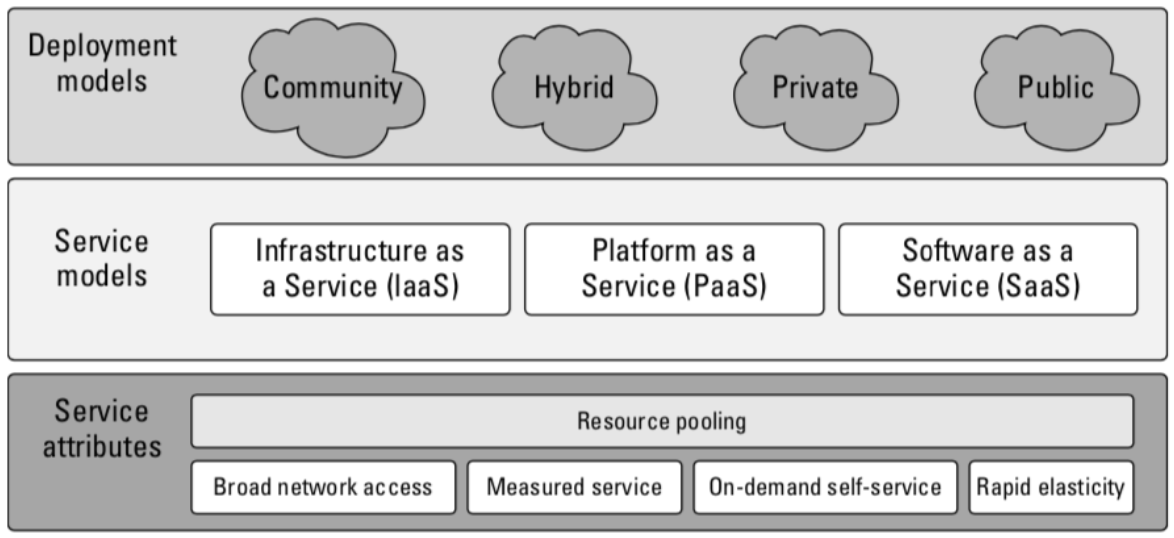
\includegraphics[width=0.8\textwidth]{assets/fig10.png}
    \caption{Cloud Computing Architecture}
    \label{fig:cloud-computing-architecture}
\end{figure}

\section{Service Attributes}

\begin{itemize}
    \item \textbf{On-demand}
    On-demand computing is a business computing
    model in which computing resources are made
    available to the user
    on an "as needed" basis.
    Rather than all at once, on-demand computing
    allows cloud hosting companies to provide their
    clients with access to computing resources as they
    become necessary.
    The on-demand computing model overcomes the
    common challenge that enterprises encountered of
    not being able to meet unpredictable, fluctuating
    computing demands efficiently.
    \item \textbf{Broad network access}
    Capabilities are available
    over the network and
    accessible through
    standard mechanisms that
    promote use by
    heterogeneous thin or
    thick client platforms
    (e.g., mobile phones,
    tablets, laptops, and
    workstations).
    \begin{figure}[H]
        \centering
        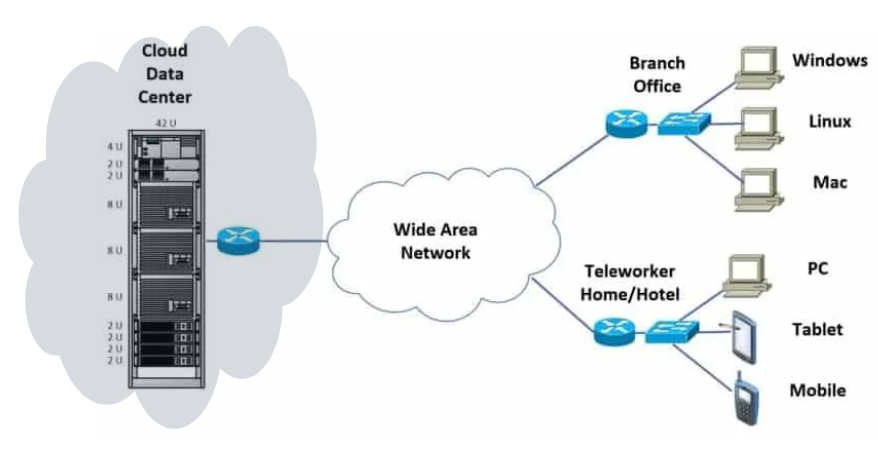
\includegraphics[width=0.8\textwidth]{assets/fig11.png}
        \caption{Broad network access}
        \label{fig:broad-network-access}
    \end{figure}
    \item \textbf{Resource pooling}
    Computing resources are storage,
    processing, memory, network
    bandwidth and virtual machines. 
    Provider’s computing resources are
    pooled to serve multiple consumers,
    allocated and deallocated as needed.
    Tenants are Isolated. Location independence: there is no
    control over the exact location of the
    resources. This has major implications
    performance, scalability, security.
    \begin{figure}[H]
        \centering
        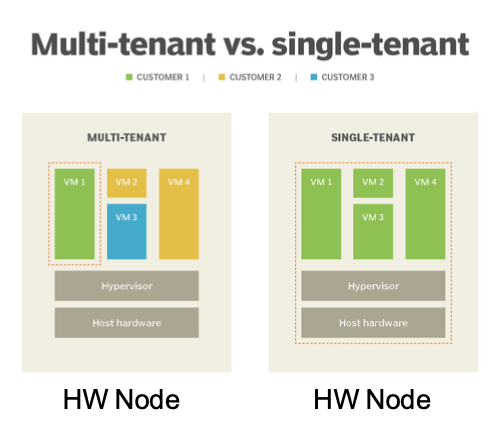
\includegraphics[width=0.5\textwidth]{assets/fig12.png}
        \caption{Resource pooling}
        \label{fig:resource-pooling}
    \end{figure}
    \item \textbf{Rapid elasticity}
    Capabilities can be elastically
    provisioned and released, in some
    cases automatically, to scale
    rapidly outward and inward
    commensurate with demand.
    To the consumer, the capabilities
    available for provisioning often
    appear to be unlimited and can be
    appropriated in any quantity at any
    time.
    \item \textbf{Vertical and horizontal scaling}
    \begin{itemize}
        \item \textbf{Vertical scaling}: adding more resources to a single node
        \item \textbf{Horizontal scaling}: adding more nodes to a system, such as adding a new computer to a distributed software application
    \end{itemize}
    \item \textbf{Measured service}
    Metering capability of service/resource abstractions in terms of storage,
    processing, bandwidth, active user accounts etc. Remember the utility computing and pay as you go model.
\end{itemize}

\section{Cloud Service Models}

\begin{itemize}
    \item \textbf{Infrastructure as a Service (IaaS)}: provides virtualized computing resources over the internet. IaaS is one of the three main categories of cloud computing services, alongside Software as a Service (SaaS) and Platform as a Service (PaaS).
    \item \textbf{Platform as a Service (PaaS)}: provides a platform allowing customers to develop, run, and manage applications without the complexity of building and maintaining the infrastructure typically associated with developing and launching an app.
    \item \textbf{Software as a Service (SaaS)}: is a software distribution model in which a third-party provider hosts applications and makes them available to customers over the internet.
\end{itemize}

\begin{figure}[H]
    \centering
    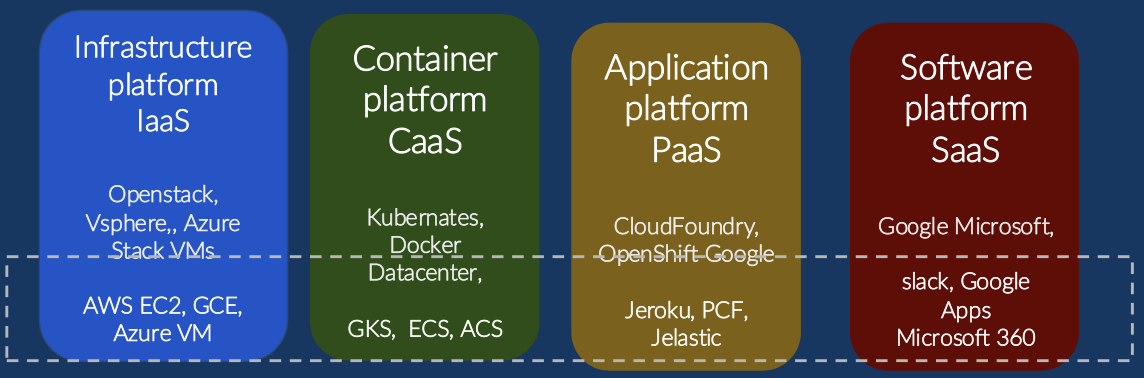
\includegraphics[width=0.8\textwidth]{assets/fig13.png}
    \caption{Cloud Service Models}
    \label{fig:cloud-service-models}
\end{figure}

\section{Cloud Deployment Models}

\begin{itemize}
    \item \textbf{Public Cloud}: The cloud infrastructure is provisioned for open use by the general public. It may be owned, managed, and operated by a business, academic, or government organization, or some combination of them. They exist on the premises of the cloud provider.
    \item \textbf{Commercial cloud}: The cloud infrastructure is provisioned for open use by the general public. It may be owned, managed, and operated by a business, academic, or government organization, or some combination of them. They exist on the premises of the cloud provider.
    \item \textbf{Hybrid cloud}: The cloud infrastructure is a composition of two or more distinct cloud infrastructures (private, community, or public) that remain unique entities but are bound together by standardized or proprietary technology that enables data and application portability (e.g., cloud bursting for load balancing between clouds).
    \item \textbf{Community cloud}: A community cloud is one where the cloud has been
    organized to serve a common function or purpose.
\end{itemize}

\section{Cloud Computing Infrastructure}

\begin{itemize}
    \item \textbf{Data Center}: A data center is a facility composed of networked computers and storage that businesses or other organizations use to organize, process, store and disseminate large amounts of data.
    \item \textbf{Virtualization}: Virtualization is the process of creating a virtual version of something, including virtual computer hardware platforms, storage devices, and computer network resources.
    \item \textbf{Hypervisor}: A hypervisor, also known as a virtual machine monitor, is a process that creates and runs virtual machines (VMs).
    \item \textbf{Containerization}: Containerization is a lightweight alternative to full machine virtualization that involves encapsulating an application in a container with its own operating environment.
    \item \textbf{Microservices}: Microservices are a software development technique—a variant of the service-oriented architecture (SOA) architectural style that structures an application as a collection of loosely coupled services.
\end{itemize}

It is based on the concept of virtualization, which allows for the creation of multiple virtual machines on a single physical machine. This allows for the efficient use of resources and the ability to scale up or down as needed. For this, Virtual Machines (VMs) are used, which are software-based representations of physical machines. These VMs can be created, modified, and deleted as needed, allowing for the efficient use of resources.

\begin{figure}[H]
    \centering
    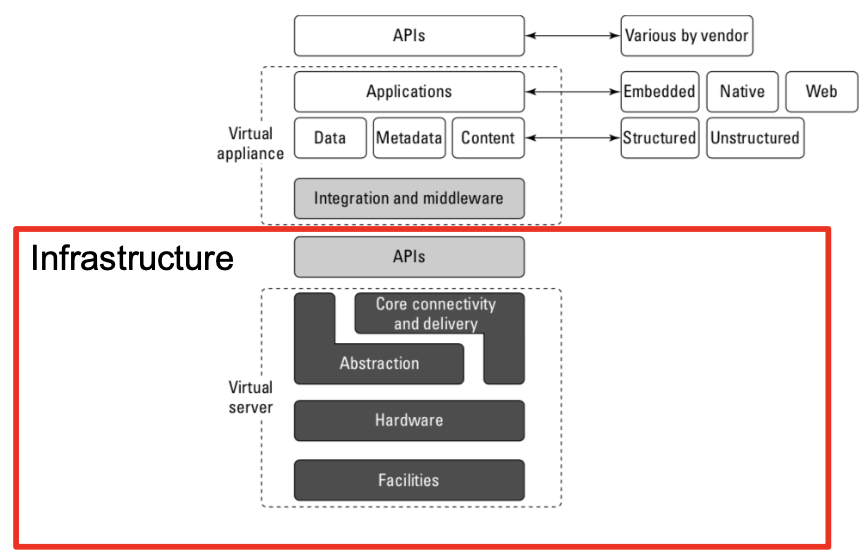
\includegraphics[width=0.8\textwidth]{assets/fig14.png}
    \caption{Cloud Computing Infrastructure}
    \label{fig:cloud-computing-infrastructure}
\end{figure}

Applications such as a Web
server or database server that
can run on a virtual machine
image are referred to as virtual
appliances. Virtual appliances are software
installed on virtual servers. They are
self-contained and run on a
virtual machine. They are
pre-configured and ready to run
applications.

\section{Communication in Cloud Computing}

Cloud computing arises from services available over the
Internet communicating using the standard Internet protocol
suite underpinned by the HTTP and HTTPS transfer
protocols.

\begin{itemize}
    \item \textbf{HTTP}: Hypertext Transfer Protocol (HTTP) is an application protocol for distributed, collaborative, hypermedia information systems. HTTP is the foundation of data communication for the World Wide Web.
    \item \textbf{HTTPS}: Hypertext Transfer Protocol Secure (HTTPS) is an extension of the Hypertext Transfer Protocol (HTTP). It is used for secure communication over a computer network and is widely used on the Internet.
    \item \textbf{REST}: Representational State Transfer (REST) is a software architectural style that defines a set of constraints to be used for creating Web services.
    \item \textbf{SOAP}: Simple Object Access Protocol (SOAP) is a messaging protocol that allows programs that run on disparate operating systems (such as Windows and Linux) to communicate using Hypertext Transfer Protocol (HTTP) and its Extensible Markup Language (XML).
\end{itemize}

\begin{observationblock}[REST]
    REST is an architectural style that defines a set of constraints to be used for creating web services. RESTful web services allow the requesting systems to access and manipulate textual representations of web resources by using a uniform and predefined set of stateless operations.
    \begin{figure}[H]
        \centering
        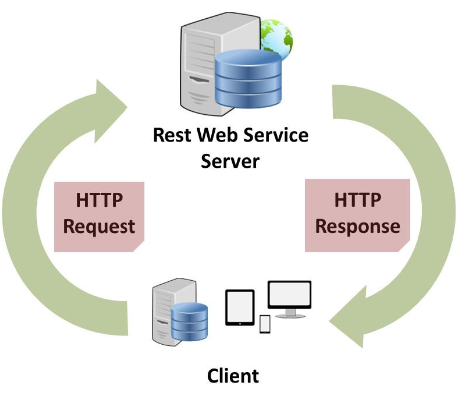
\includegraphics[width=0.5\textwidth]{assets/fig15.png}
        \caption{REST}
        \label{fig:rest}
    \end{figure}
\end{observationblock}

Advantages of REST:
\begin{itemize}
    \item \textbf{Scalability}: RESTful web services can be scaled to accommodate a large number of clients.
    \item \textbf{Performance}: RESTful web services are faster than SOAP web services because they are usually written in a lightweight language like JSON.
    \item \textbf{Simplicity}: RESTful web services are easier to understand and implement than SOAP web services.
    \item \textbf{Flexibility}: RESTful web services can be used with any programming language and can be easily integrated with other web services.
\end{itemize}

REST implementation:
\begin{enumerate}
    \item Identify all the conceptual entities that we wish to expose as services. 
    \item Create a URL to each resource.
    \item Categorize our resources according to whether clients can just receive a representation of the resource or whether clients can modify the resource.
    \item All resources accessible via HTTP GET should be side-effect free, i.e., the resource should just return a representation of the resource (not modify it).
    \item Put hyperlinks in the representation of the resource to allow clients to navigate to related resources.
    \item Design to reveal data gradually. Don't reveal anything in a single response document. Provide hyperlinks to obtain mode details. 
    \item Specify the format of response datausing a schema (DTD, W3C Schema, RelaxNG, ...). For those services that require a POST or PUT to it, also provide a schema to specify the format of the response. 
    \item Describe how our services are to be invoked using either a WSDL document or simply an HTML document. 
\end{enumerate}